\chapter{Flexible Regularization for CCA}
\label{chap:als}
\minitoc

\section{Introduction}\label{sec:introduction}

This chapter is an extension of work that I have previously presented in poster form at the OHBM conference.
I have benefitted from constructive theoretical discussions with John Shawe-Taylor and Janaina Mourao-Miranda, as well as insights into result interpretation from Janaina and Rick Adams.

The core focus of this part of my PhD research shifts towards understanding and improving the regularization in Canonical Correlation Analysis (CCA) models.
Traditional CCA models often exhibit shortcomings when grappling with high-dimensional data, a challenge particularly acute in the context of brain-behavior studies.
In response, this chapter introduces Flexible Regularized Alternating Least Squares (FRALS), an optimized framework for regularized CCA.

\subsection{Problem Statement}\label{subsec:problem-statement}

Classical CCA methods struggle with high-dimensional data, leading to problems like overfitting and spurious conclusions.
We aim to investigate the role of model priors in CCA by using simulated and real data to show that the best model performance is achieved when the model priors match the data-generating priors.
Further, we delve into the implications of regularizing weights and loadings, arguing that regularized weights may
improve out-of-sample correlation but are less interpretable than loadings.

\subsection{Contributions}\label{subsec:contributions}

This chapter brings several contributions to the field of multiview machine learning and specifically to the application of CCA in brain-behavior studies.
First, we review existing methods for generating simulated data in CCA research and propose a new method based on the probabilistic model of CCA. We use this to justify focusing on the comparison of loadings rather than weights.
Second, we introduce FRALS, a novel and flexible framework that allows for the utilization of any regularized least squares solver, thereby offering a more robust defense against overfitting.
Our experimental results demonstrate that FRALS shows promise in terms of out-of-sample correlation but also reveal its computational limitations, serving as an educational stepping stone for future work in this area.


\section{Background}\label{sec:background}

\subsection{How is CCA and PLS Data Generated and Why Should We Care?}\label{sec:how-is-cca-and-pls-data-generated-and
-why-should-we-care?}

Understanding the data generation process in Canonical Correlation Analysis (CCA) and Partial Least Squares (PLS) is pivotal for many reasons. It influences the choice of appropriate models, evaluation metrics, and sheds light on the underlying structure and dependencies between views. Probabilistic formulations provide a principled framework to understand this process, helping us gauge the assumptions we make and the limitations these impose.

\subsubsection{Probabilistic CCA}

In Probabilistic CCA~\cite{bach2005probabilistic}, the generative model is articulated as a two-step process for each view \(i\):

\begin{align}
    \mathbf{z}& \sim \mathcal{N}(\mathbf{0}, \mathbf{I})                                            \\
    \mathbf{x}_i & \sim \mathcal{N}(\mathbf{W}_i \mathbf{z} + \boldsymbol{\mu}_i, \boldsymbol{\Psi}_i)
\end{align}

Here, \(\mathbf{z}\) represents the latent variables shared between the different views. \(\mathbf{x}_i\) is generated conditionally based on \(\mathbf{z}\), and can be thought of as the observed data with additional noise \(\boldsymbol{\Psi}_i\).

% TikZ Diagram for Probabilistic CCA
\begin{tikzpicture}
    % Define nodes
    \node[latent] (z) {z};
    \node[obs, below=of z] (x1) {\(x_1\)};
    \node[obs, right=of x1] (x2) {\(x_2\)};
    % Connect nodes
    \edge {z} {x1,x2} ;
    % Plates
    \plate {} {(x1)(x2)} {Views}
\end{tikzpicture}

\subsubsection{Probabilistic rCCA}

Probabilistic rCCA~\cite{de2003regularization} extends Probabilistic CCA by incorporating regularization directly into the covariance structure:

\begin{align}
    \mathbf{z}& \sim \mathcal{N}(\mathbf{0}, \mathbf{I})                                            \\
    \mathbf{x}_i & \sim \mathcal{N}(\mathbf{W}_i \mathbf{z} + \boldsymbol{\mu}_i, \boldsymbol{\Psi}_i + \Sigma_i^2)
\end{align}

Here, \(\Sigma_i^2\) is a diagonal matrix that models measurement noise. This addition allows the model to be more robust to overfitting and other data challenges.

\subsubsection{Probabilistic PLS}

Probabilistic formulations of PLS are still an evolving field \cite{el2018probabilistic,zheng2016probabilistic}.
Despite various models for PLS regression, a canonical probabilistic model for Canonical PLS remains elusive.
We will address this gap in our contributions.

\subsection{Forward and Backward Models}

At this stage we can consider the difference between forward and backward models in the context of CCA and PLS.
In forward models we generate data from a known model and then try to recover the parameters of that model.
In backward models we try to recover the parameters of a model from the data.

In the CCA and PLS models described in chapter \ref{chap:background} we have backward models which aim to infer the
latent variables $\bold{Z}$ from the data $\bold{X_i}$.
In the probabilistic models described in section \ref{subsec:probabilistic-cca-rcca-and-pls} we have forward models which
generate data from the latent variables $\bold{Z}$.

\subsection{Why is this important?}

If we are solely interested in the latent variables $\boldsymbol{Z}$, then the backward models described in chapter \ref{chap:background} suffice for inferring them from the data. However, if we aim for a comprehensive understanding and interpretability of the model, it becomes vital to understand both forward and backward formulations.

Consider the probabilistic CCA model described in section \ref{subsec:probabilistic-cca-rcca-and-pls}, but with concrete names for the latent variables and views. Let's take figure \ref{fig:mentalhealthselfsupervised} as an example where the latent variable represents the severity of a mental health condition, and the views (neuroimaging and behavioral data) are conditioned on this latent variable.


\begin{figure}
    \centering
    \tikz{
        % nodes
        \node[latent, align=center, minimum size=2cm] (Z) {Severity};
        %
        \node[obs, below left=of Z, minimum size=2cm] (X_1) {Neuroimage};%
        \node[obs, below right=of Z, minimum size=2cm] (X_2) {Behaviour};%
        % edges
        \edge{Z} {X_1}
        \edge{Z} {X_2}}
    \caption[Latent Variable Model of Mental Health]{\textit{\textbf{Latent Variable Model of Mental Health:}} From this perspective the neuroimaging modality and behavioural data are both considered to have been generated with distributions conditioned on the severity of a mental health condition}\label{fig:mentalhealthselfsupervised}
\end{figure}

In both the forward and backward models of CCA, the latent variables are of interest and are mathematically identifiable (up to a rotation), meaning that although they may be represented differently, they capture the same underlying structure. However, their conceptual implications differ between the two models. In the forward model, the weights indicate how the latent variables influence the generation of the views. Conversely, in the backward model, the weights help us best predict or reconstruct the latent variables from the data.

\subsection{What is the relationship between the forward and backward weights?}

Both the forward and backward models of CCA give analytical forms for the joint covariance matrix of the views.

\begin{align}
    \Sigma &= \begin{bmatrix}
        \bold{W_1W_1^T} + \bold{\Psi_1} & \bold{W_1W_2^T} \\
        \bold{W_2W_1^T} & \bold{W_2W_2^T} + \bold{\Psi_2}
    \end{bmatrix} = \begin{bmatrix}
        \bold{\Sigma_1} & \bold{\Sigma_1}\sum_k \rho_k u_{1_k}^\top u_{2_k} \bold{\Sigma_2}  \\
        \bold{\Sigma_2}\sum_k \rho_k u_{2_k}^\top u_{1_k} \bold{\Sigma_1} & \bold{\Sigma_1}
    \end{bmatrix}
\end{align}

Where $\rho_k$ is the $k$th canonical correlation and $u_{i_k}$ is the $k$th column of $\bold{U_i}$.

By examining the joint covariance matrix we can see that the weights in the forward model are related to the weights in the backward model by:

\begin{align}
    \bold{W_1W_2^T} &= \bold{\Sigma_1}\sum_k \rho_k u_{1_k}^\top u_{2_k} \bold{\Sigma_2}
\end{align}

For a single latent variable, we therefore have:

\begin{align}
    \bold{w_1} &= p_1\bold{\Sigma_1} u_{1_1}^\top \\
    \bold{w_2} &= p_2\bold{\Sigma_2} u_{2_1}^\top
\end{align}

Where $p_i$ is a scalar constant and $\prod_i p_i = \rho$. Notice that the weights in the backward model are scaled
by the covariance matrices $\bold{\Sigma_i}$ so this is almost exactly the same definition as loadings.

Note that weights in forward and backward models are the same (up to scaling by $p$) if the covariance matrices are identity matrices.
Further note that sparse weights do not in general imply sparse loadings and vice versa (unless the covariance matrices are identity matrices).

\subsection{Data Generation}\label{subsec:data-generation-background}

There are a number of ways used in the Sparse CCA literature to generate synthetic data.
Witten\cite{witten2009extensions} used a generative model of the form defined by:

\begin{align}\label{eq:wittengen}
    & \bold{X_i}=\bold{z_kw_{ki}}+\epsilon
\end{align}

which we can represent as the graphical model in figure~\ref{fig:wittengraphical}.

While this simple method directly controls the cross-covariance it doesn't control the within dataset covariance $\bold{\Sigma_{ii}}$.
Later papers in the sparse CCA literature such as~\cite{mai2019iterative,chen2013sparse} have constructed the covariance matrix as in figure~\ref{fig:covariance} and sampled from this multivariate normal distribution to give two simulated views with specified active variables, correlations and within-view covariance.
This has the advantage of allowing us to control the within-view covariance and therefore test the methods under specific conditions.
The process was first described by Chen~\cite{chen2013sparse} and further explained by~\cite{suo2017sparse}.


\section{A generative model for canonical PLS}\label{subsec:a-generative-model-for-canonical-pls}

Our first contribution is to show that the data generation process described in~\cite{witten2009extensions} actually
allows us to define a probabilistic model for latent variable PLS. The data generation process in equation \ref{eq
:wittengen} is equivalent to the graphical model in figure~\ref{fig:wittengraphical}.

\begin{figure}
\centering
  \tikz{
%nodes
 \node[latent, align=center] (Z) {$Z$}; %
 \node[obs, below left=of Z] (X_1) {$X_1$};%
 \node[obs, below right=of Z] (X_2) {$X_2$};%
 \node[latent,above left=of X_1,fill] (W_1) {$W_1$}; %
 \node[latent,above right=of X_2,fill] (W_2) {$W_2$}; %
 \node[latent,left=of X_1] (sigma_1) {$\sigma_1$}; %
 \node[latent,right=of X_2] (sigma_2) {$\sigma_2$}; %
% edges
 \edge {W_1,Z,sigma_1} {X_1}
 \edge {W_2,Z,sigma_2} {X_2}}
 \caption[Sparse Data Generation Graphical Model]{\textit{\textbf{Sparse Data Generation Graphical Model: }}For the Witten data generation, we set the active variables with the matrices $W_i$ and therefore rescale the latent variable Z in those variables with zeros in the other variables. Z has standard normal distribution. We add gaussian noise parameterized by $\sigma$.}
 \label{fig:wittengraphical}
\end{figure}

By marginalizing out the latent variable $Z$ we can write down the joint distribution of the two views as:

\begin{align}
    p(X_1,X_2) &= \int p(X_1,X_2,Z) dZ \\
    &= \int p(X_1|Z)p(X_2|Z)p(Z) dZ \\
    &= \int \mathcal{N}(X_1|W_1Z,\sigma_1^2) \mathcal{N}(X_2|W_2Z,\sigma_2^2) \mathcal{N}(Z|0,1) dZ
\end{align}

Which means the joint covariance matrix is given by:

\begin{align}
    \Sigma &= \begin{bmatrix}
        W_1W_1^T + \sigma_1^2I & W_1W_2^T \\
        W_2W_1^T & W_2W_2^T + \sigma_2^2I
    \end{bmatrix}
\end{align}

Where analagously to probabilistic PCA\cite{tipping1999probabilistic}, we recover PLS by setting $\sigma_1^2 = \sigma
_2^2 = 0$.
To the best of our knowledge, this is the first probabilistic model for the canonical PLS models described in this
thesis.

% Likelihood Function
\begin{align*}
\mathcal{L}(W_1, W_2 | X_1, X_2) &= \prod_{i=1}^{N} p(\mathbf{x}_{1i}, \mathbf{x}_{2i}) \\
&= \prod_{i=1}^{N} \frac{1}{(2\pi)^{d/2} |C|^{1/2}} \exp \left( -\frac{1}{2} (\mathbf{x}_i - \boldsymbol{\mu})^T C^{-1} (\mathbf{x}_i - \boldsymbol{\mu}) \right)
\end{align*}

% Log-Likelihood Function
\begin{align*}
\log \mathcal{L}(W_1, W_2 | X_1, X_2) &= -\frac{Nd}{2} \log(2\pi) - \frac{N}{2} \log |C| - \frac{1}{2} \sum_{i=1}^{N} (\mathbf{x}_i - \boldsymbol{\mu})^T C^{-1} (\mathbf{x}_i - \boldsymbol{\mu})
\end{align*}

% Optimization
\begin{align*}
W_1^*, W_2^* = \arg\max_{W_1, W_2} \log \mathcal{L}(W_1, W_2 | X_1, X_2)
\end{align*}

% Sample covariance
\begin{align*}
S &= \frac{1}{N} \sum_{i=1}^N (\mathbf{x}_i - \boldsymbol{\mu})(\mathbf{x}_i - \boldsymbol{\mu})^T
\end{align*}

% Relate C and S
Note that in practice, \( C \) would often be estimated as the sample covariance matrix \( S \) which would then be factorized to obtain \( W_1 \) and \( W_2 \).



\subsection{}

\section{Flexible Regularized Alternating Least Squares (FRALS)}\label{subsec:flexible-regularized-alternating-least-squares-(frals)}
We adopt an alternating minimization strategy to solve the CCA problem.
The objective is to minimize the sum of squared Frobenius norms between the latent variables and their projections in each view.
Regularization terms are added to the objective function to avoid overfitting.
Our formulation allows the incorporation of any regularized least squares solver, making it extremely flexible.

\subsection{Mathematical Formulation}
We can solve CCA by alternating minimization over each view, based on the alternating least squares form.
This form finds a variable \( T \) that is close to the latent variables \( X\sps{1} U\sps{1} \), where \( X\sps{1} \), \( U\sps{1} \) are the matrix and weights for each view \( i \).
The closer \( T \) is to \( X\sps{1} U\sps{1} \), the higher the correlation between them.
The constraint \( T^\top T = I \) ensures that the latent space is orthogonal to find different effects.

\begin{gather*}
    \underset{U, T}{\mathrm{argmin}}\left\{\sum_i \|X\sps{i} U\sps{i} - T\|_F^2 \right\}\\
    \text{subject to: } T^\top T = I\\
\end{gather*}

To regularize the projection matrices, we add penalty terms to the objective function, such as \( P(U\sps{1}) = \lambda_i \|U\sps{1}\|_F \) for ridge regression or \( P(U\sps{1}) = \lambda_i \|U\sps{1}\|_1 \) for lasso.
This can help us avoid overfitting and improve the interpretability of the results.
This means that \textbf{any regularized least squares solver} can be used to solve each subproblem, such as ridge regression, lasso, elastic net, etc., making our framework substantially more flexible than prior work.

\begin{gather*}
    \underset{U, T}{\mathrm{argmin}}\left\{\sum_i \|X\sps{i} U\sps{i} - T\|_F^2 + \textcolor{red}{\lambda_i P(U\sps{i})}\right\}\\
    \text{subject to: } T^\top T = I\\
\end{gather*}


\section{Experiment 1: Simulated Data Evaluation}\label{subsec:exp1}

In this experiment, we evaluate several Sparse Canonical Correlation Analysis (CCA) variants using synthetic data generated with the FRALS framework.

Two of these variants, IPLS+ and ElasticNet, are implemented within the FRALS framework for added flexibility.
We provide intuition for the comparison of these models:

- \textbf{IPLS+ (Sparse CCA via Iterative Penalized Least Squares with Positive Constraints):} IPLS+ assumes a prior about the data generation process, specifically that the true weights are positive.
This prior matches the data generation process, making it more suitable for the given synthetic data.
As a result, IPLS+ is expected to perform well as it aligns with the underlying data structure.

- \textbf{ElasticNet:} ElasticNet, another model implemented using the FRALS framework, offers a combination of L1 (lasso) and L2 (ridge) regularization.
While it provides flexibility in handling different types of data, it may not align with the specific prior assumption of positive weights in our synthetic data generation process.

\subsubsection{Simulated Data Generation}\label{subsubsec:simulated-data-generation}

In this experiment, we evaluate several Sparse Canonical Correlation Analysis (CCA) variants using synthetic data generated with the FRALS framework. Two of these variants, IPLS+ and ElasticNet, are implemented within the FRALS framework for added flexibility.

Therefore, we anticipate that IPLS+ may outperform ElasticNet due to its alignment with the prior assumptions about data generation. This experiment aims to validate this intuition by comparing the performance of these models and others.

\subsubsection{Methodology}

To carry out the experiment, we leverage the CCA-Zoo Python package. The synthetic data is generated using the \texttt{LinearSimulatedData} class from the package, with parameters set to emulate a high-dimensional feature space.

\begin{table}[h]
\centering
\caption{Experiment Parameters}
\begin{tabular}{l|l}
\textbf{Parameter} & \textbf{Value} \\
\hline
Number of samples (\textit{n}) & 500 \\
Number of features in View 1 (\textit{p}) & 200 \\
Number of features in View 2 (\textit{q}) & 200 \\
Latent dimensions & 1 \\
Sparsity in View 1 & 0.1 \\
Sparsity in View 2 & 0.1 \\
Target correlation between views & 0.9 \\
\end{tabular}
\label{table:experiment-parameters}
\end{table}

We employ several CCA variants for this experiment:

\begin{table}[h]
\centering
\caption{Employed CCA Variants}
\begin{tabular}{l}
\textbf{CCA Variant} \\
\hline
Canonical Correlation Analysis (CCA) \\
Partial Least Squares (PLS) \\
Sparse CCA via Penalized Majorization-Minimization (SCCA\_PMD) \\
Sparse CCA via Iterative Penalized Least Squares (SCCA\_IPLS) \\
Sparse CCA via Span Regularization (SCCA\_Span) \\
Elastic CCA \\
\end{tabular}
\label{table:cca-variants}
\end{table}

Grid search is used for hyperparameter tuning for Elastic CCA and SCCA\_PMD models.

\subsubsection{Evaluation Metrics}

The models are evaluated based on their correlation score on a validation set comprising 20\% of the original data. Additionally, the weights of each model are visualized for interpretability.

\section{Results and Discussion}

\subsection{Performance Comparison}

\subsection{True Weights for Context}

Figure~\ref{fig:True_weights} provides a ground truth reference for the weights in the true underlying signal, setting the context for our subsequent analysis.

\begin{figure}[h]
    \centering
    \includesvg[width=0.6\textwidth]{figures/als/simulated/True_weights.svg}
    \caption{Ground truth weights for the true underlying signal.}
    \label{fig:True_weights}
\end{figure}

\subsection{Interpretation of Weight Plots}

Figures~\ref{fig:CCA_weights} to~\ref{fig:IPLS+_weights} visualize the weights attributed to each feature by different models.
Different colors indicate the indices of weights involved in the true signal (as shown in Figure~\ref{fig:True_weights}) and those not involved.

\subsection{Performance Insights}

\paragraph{Impact of Sparsity:}
Figure~\ref{fig:PLS_weights} and Figure~\ref{fig:CCA_weights} display the weights for PLS and CCA, respectively.
Both models lack sparsity priors and hence select all features with non-zero weights.
This dilutes the true signal and results in lower validation correlation.

\begin{figure}[h]
    \centering
    \includesvg[width=0.6\textwidth]{figures/als/simulated/PLS_weights.svg}
    \caption{PLS selects all features with non-zero weights, leading to diluted true signals.}
    \label{fig:PLS_weights}
\end{figure}

\begin{figure}[h]
    \centering
    \includesvg[width=0.6\textwidth]{figures/als/simulated/CCA_weights.svg}
    \caption{ Similar to PLS, CCA also lacks a sparsity prior, leading to poor feature selection.}
    \label{fig:CCA_weights}
\end{figure}

\paragraph{Objective Mismatch:}
In contrast, PMD incorporates a sparsity prior. However, as seen in Figure~\ref{fig:PMD_weights}, its objective is to maximize covariance, not correlation. This leads to its middling performance.

\begin{figure}[h]
    \centering
    \includesvg[width=0.6\textwidth]{figures/als/simulated/PMD_weights.svg}
    \caption{PMD shows sparsity but focuses on maximizing covariance rather than correlation.}
    \label{fig:PMD_weights}
\end{figure}

\paragraph{Efficacy of IPLS:}
IPLS performs well due to its alternating lasso procedure and sparsity priors on each view. Figure~\ref{fig:IPLS_weights} confirms its ability to better capture the true underlying signal.

\begin{figure}[h]
    \centering
    \includesvg[width=0.6\textwidth]{figures/als/simulated/SCCA_IPLS_weights.svg}
    \caption{IPLS captures the true underlying signal effectively, thanks to its sparsity priors.}
    \label{fig:IPLS_weights}
\end{figure}

\paragraph{Advantage of Elastic Net:}
Elastic Net regularization combines both $l_1$ and $l_2$ penalties. As Figure~\ref{fig:ElasticNet_weights} shows, this strikes a good balance between feature selection and signal capture.

\begin{figure}[h]
    \centering
    \includesvg[width=0.6\textwidth]{figures/als/simulated/ElasticCCA_weights.svg}
    \caption{Elastic Net shows balanced feature selection and effective signal capture.}
    \label{fig:ElasticNet_weights}
\end{figure}

\paragraph{Superiority of IPLS+:}
As illustrated in Figure~\ref{fig:IPLS+_weights}, IPLS+ with a positive constraint shows the best performance among the models tested, emphasizing the benefit of domain-specific priors.

\begin{figure}[h]
    \centering
    \includesvg[width=0.6\textwidth]{figures/als/simulated/SCCA_IPLS_positive_weights.svg}
    \caption{IPLS+ outperforms other models, benefiting from a positive constraint.}
    \label{fig:IPLS+_weights}
\end{figure}

\subsection{Conclusion}

The experimental results underscore the importance of incorporating sparsity and other domain-specific priors in multiview learning models.
The interleaved figures and discussions affirm the need to align the model's objective with the characteristics of the underlying signal for effective feature selection and signal capture.




\subsection{Experiment 2: Human Connectome Project (HCP) Data Evaluation}

\subsubsection{Experiment Design}
In our study, we used resting-state fMRI along with non-imaging subject measures from a total of 1003 healthy subjects, sourced from the 1200-subject data release of the Human Connectome Project (HCP). The dataset was divided into an 80\% training set and a 20\% testing set.
To fine-tune the regularization of hyperparameters, cross-validation was employed within the training data.
Our approach, dubbed Flexible Regularized Alternating Least Squares (FRALS) with elastic net regularization on both views, was compared against existing methods, namely separate PCA on each modality, Penalized Matrix Decomposition (PMD), and Ridge Regularized CCA (RCCA). The performance was evaluated based on out-of-sample correlations.

\subsubsection{Performance Metrics}
The primary metric for evaluating the performance of our FRALS model was out-of-sample canonical correlations.
It was compared against PCA performed individually on each modality, as well as against PMD and RCCA\@.

\subsubsection{Performance Metrics}
Our model, FRALS, demonstrated superior performance by achieving the highest out-of-sample canonical correlations among all models tested (see Figure~\ref{fig:performance}).

\begin{figure}[h]
\centering
\includesvg[width=0.5\linewidth]{figures/als/hcp/barcorr}
\caption{Out-of-sample canonical correlations for each model.}
\label{fig:performance}
\end{figure}

\subsubsection{Model Similarities}
We computed the correlation matrix of the scores for each modality to evaluate the similarity of the latent variables learned by each model.
FRALS exhibited low or negative correlations with other models, highlighting its ability to capture novel and distinct aspects of brain-behaviour associations (see Figure~\ref{fig:similarities}).

\begin{figure}[h]
\centering
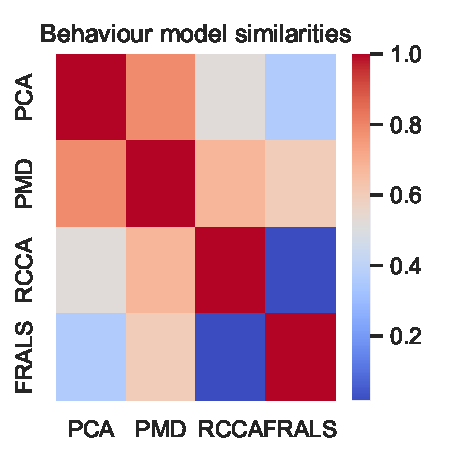
\includegraphics[width=0.49\linewidth]{figures/als/hcp/behaviour_model_similarities}
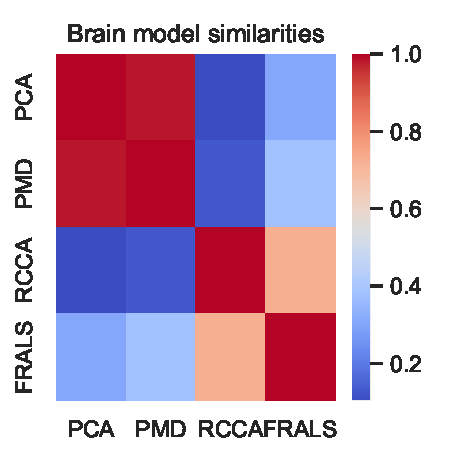
\includegraphics[width=0.49\linewidth]{figures/als/hcp/brain_model_similarities}
\caption{Left: Correlation matrix of the scores for each modality. Right: Correlation matrix of the brain loadings for each model.}
\label{fig:similarities}
\end{figure}


\subsubsection{Behaviour and Brain Loadings}
In terms of behavioral loadings, except for PCA, all models identified a latent variable that correlated positively with cognitive tests and negatively with cigarette, tobacco, or alcohol use.
Both RCCA and FRALS demonstrated stronger correlations with the Line Orientation test, which measures visuospatial abilities.

\begin{figure}[h]
\centering
\includesvg[width=\linewidth]{figures/als/hcp/all_top_and_bottom_loadings.svg}
\caption*{Top 5 positive and negative non-imaging loadings for each model}
\label{fig:behaviour}
\end{figure}

Regarding the brain loadings, our analysis shows that each model assigns different weights to various brain regions
based on their connectivity.
RCCA and FRALS assigned more weight to the parietal lobe, known for its role in visuospatial processing, than did PCA and PMD. This suggests that the parietal lobe is more relevant for the brain-behaviour correlations captured by our model.
Conversely, PMD appears to rely on principal components in the brain, potentially missing the true associations between the views.
FRALS functions as a sparse version of RCCA in this context.

\begin{figure}[h]
\centering
\includegraphics[width=0.49\linewidth]{figures/als/hcp/pca_brain_loadings}
\includegraphics[width=0.49\linewidth]{figures/als/hcp/pmd_brain_loadings}
\includegraphics[width=0.49\linewidth]{figures/als/hcp/rcca_brain_loadings}
\includegraphics[width=0.49\linewidth]{figures/als/hcp/flexals_brain_loadings}
\caption*{Map of CCA connection strength increases/decreases, with each node’s parcel map weighted by CCA edge-strength increases, summed across edges involving that node.}
\label{fig:brain}
\end{figure}

\section{Discussion}


\section{Limitations}\label{sec:limitations}

While FRALS offers promising performance in terms of out-of-sample correlation, it does come with significant drawbacks, the most noteworthy being its computational inefficiency. Below, we outline the primary factors contributing to the slow speed of FRALS and provide some insights into the computational bottlenecks.

\subsection{Computational Time}\label{subsec:computational-time}
One of the major constraints of FRALS is the time complexity involved in solving the regularized least squares regressions to completion. The algorithm’s iterative nature, which involves solving a sequence of regressions, makes it computationally intensive, particularly when dealing with high-dimensional data.

\subsection{Changing Regression Targets}\label{subsec:changing-regression-targets}
Adding to the computational burden is the fact that the regression targets, i.e., the projections of the other view, are not static but change dynamically throughout the algorithm's run.
Each update to the least squares solution consequently alters the global objective, leading to a constantly shifting landscape that the algorithm needs to navigate.





\subsection{Conclusions and Further Work}
The main idea of this chapter is to introduce FRALS, a novel approach in the realm of multiview learning that optimizes
both flexibility and performance.
Our experiments indicate that FRALS not only outperforms established methods like PCA, PMD, and RCCA in terms of out-of-sample canonical correlations but also captures novel and distinct aspects of brain-behavior associations.
This uniqueness is evident from the low or negative correlations FRALS holds with other models.

Our findings also underline the importance of the parietal lobe in understanding brain-behavior associations.
FRALS emphasizes this region more compared to traditional methods like PCA and PMD. Future work should focus on understanding the specific functions and contributions of different brain regions captured by FRALS and how they relate to various behaviors.

Given its promising initial results, the next step for FRALS would be its application to larger datasets and its adaptation for different kinds of biological and non-biological data to further evaluate its robustness and applicability.



\section{Conclusion}

We have introduced a flexible and efficient framework for regularized CCA that addresses the limitations of existing methods.
Our framework is particularly well-suited for high-dimensional data and can be adapted to various types of regularization, offering an effective tool for uncovering complex relationships in multiview data.







